Klient aplikacji ma dwa główne zadanie --- rysowanie widgetów aplikacji z zachowaniem hierarchii oraz zbieranie zdarzeń \emph{DOM} takich jak kliknięcia na widgety, wciśnięcie klawiszy. Do komunikacji używana jest technologia \emph{WebSocket}. Rysunek \ref{fig:arch-render} przedstawia architekturę klienta.

Zdarzenia \emph{DOM} zbierane są z całości dokumentu. W przypadku zdarzeń myszy na podstawie pozycji następuje przyporządkowanie do elementu znajdującego się pod kursorem. Zebrane dane zamieniane są na obiekt \emph{JSON} rozumiany przez serwer i wysyłane do niego.

Do rysowania widgetów w dokumencie używane są dane wysyłane przez serwer. Przeglądarka nasłuchuje na połączeniu \emph{WebSocket} na polecenia sterujące w formacie \emph{JSON} i wykonuje je rysując na elemencie \emph{canvas} lub manipulując odpowiednio drzewem \emph{DOM}, np. otwierając nowe okno, lub chowając dany widget. Obrazy nie są przesyłane bezpośrednio. W obiektach sterujących \emph{JSON} znajdują się jedynie klucze pozwalające na jednorazowe pobranie obrazu z serwera obrazów w celach optymalizacyjnych.

\begin{figure}[H]
\centering
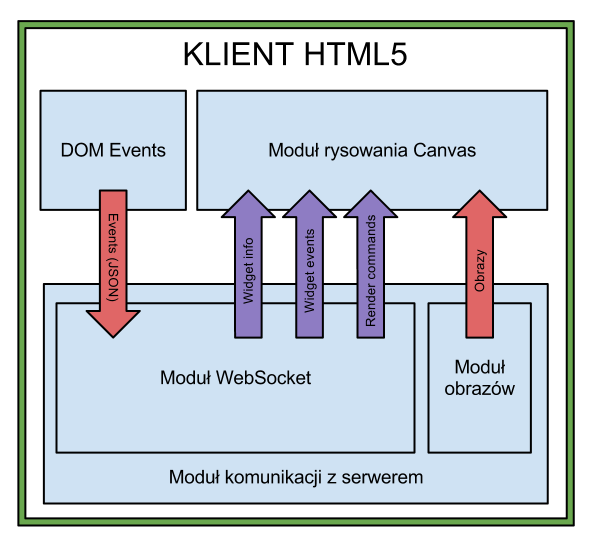
\includegraphics[width=0.8\linewidth]{img/arch-render}
\caption{Schemat architektury odtwarzania wyglądu aplikacji po stronie klienta.}
\label{fig:arch-render}
\end{figure}
